\section{The charged upper-area inequality}
\label{ch:intro:charged-section}

We now extend the neutral exterior inequality to divergence-free electric and magnetic fields with neutral exterior matter satisfying the physical dominant energy condition. In the presence of charge, the numerical statement is an upper bound for the area radius,
\begin{equation}\label{ch:intro:bound}
 r\le m+\sqrt{m^2-Q^2},\qquad m\ge Q,
\end{equation}
where $Q$ is the magnitude of the total charge and $m$ is the invariant ADM mass. For disconnected horizons, it is essential to retain this upper-bound formulation: the familiar expression $(r+Q^2/r)/2$ is not increasing throughout the positive $r$-axis. Khuri--Weinstein--Yamada developed a charged conformal-flow approach for multiple horizon components \cite{KhuriWeinsteinYamada2017}; the distinction between the two area branches is already visible in the counterexamples of Weinstein--Yamada \cite{WeinsteinYamada2005}.

For non-time-symmetric data, Disconzi--Khuri developed electric graph transport preserving charge and divergence, and a reduction conditional on a coupled Jang--inverse-mean-curvature-flow system \cite{DisconziKhuri2012}. We combine the neutral construction above with the charged numerical theorem of the companion paper \cite[Theorem~2.3]{ChargedOriginalData2026}. Proposition~\ref{ch:pre:neutral-exterior} transfers the one-sided exterior inequality to the charged notation; Proposition~\ref{ch:ell:neutral-input} transfers the elliptic construction and its estimates. Their proofs identify the precise neutral results and verify the normalizations. The charged preparation satisfies the elliptic hypotheses by Lemma~\ref{ch:ell:hypothesis-check}.

Theorem~\ref{ch:intro:main} also excludes a non-timelike ADM vector for a
nonempty smooth compact obstacle. Physical matter DEC implies total DEC,
so the endpoint corollary already proved for neutral exteriors applies;
Lemma~\ref{ch:rest:timelike} verifies its hypotheses here.

\begin{figure}[htbp]
\centering
\begin{tikzpicture}[x=1.5cm,y=1.5cm]
 \fill[black!7] (0,1)--(1,1)--
   plot[domain=1:4,samples=80] (\x,{(\x+1/\x)/2})
   --(4,2.6)--(0,2.6)--cycle;
 \draw[->] (0,0)--(4.25,0) node[right] {$r/Q$};
 \draw[->] (0,0)--(0,2.85) node[above] {$m/Q$};
 \draw[thick] (0,1)--(1,1);
 \draw[thick,domain=1:4,samples=80] plot (\x,{(\x+1/\x)/2});
 \draw[densely dotted] (1,0)--(1,2.6);
 \draw (1,.04)--(1,-.04) node[below] {$1$};
 \draw (.04,1)--(-.04,1) node[left] {$1$};
 \node at (1.95,2.15) {allowed region};
 \node[below right] at (2.4,1.18) {$m=\tfrac12(r+Q^2/r)$};
 \node[above] at (.5,1) {$m=Q$};
\end{tikzpicture}
\caption{The charged upper-area inequality for $Q>0$.
For $r\le Q$, it requires only $m\ge Q$.
For $r\ge Q$, its boundary is $m=(r+Q^2/r)/2$.
The mass-lower-bound expression must therefore be restricted to this latter branch.}
\label{fig:charged-region}
\end{figure}


Two ingredients carry the charge through the neutral construction. First, we represent the fields by closed flux two-forms and keep those forms through an annular replacement, a change to a rest end, and conformal repairs. This produces strict data whose rest energies approach the original invariant mass and whose enclosing areas approach the original infimum. The quantitative repair uses only the stated weak asymptotic derivative bounds on the original data. Second, after aligning the total charge by a constant electromagnetic rotation, a pointwise square completion controls the graph norm of one closed two-form. The other rotated form has zero total charge. This single-form comparison accommodates the electromagnetic momentum density and makes the original neutral elliptic system sufficient.

The proof proceeds through four geometric stages. Section~\ref{ch:rest:section} constructs strict charged rest data. Section~\ref{ch:prep:section} prepares their exterior boundary with a positive matter margin. Sections~\ref{ch:ell:section}--\ref{ch:mass:section} use the specified neutral system to produce Riemannian comparison metrics with the same total charge, no smaller enclosing area, and a controlled energy. Section~\ref{ch:final:section} derives their Riemannian endpoint from the companion charged numerical theorem and removes the parameters in their prescribed order.
